\section{Planificación temporal}
\subsection{Estructura de descomposición del trabajo/Planificación temporal}
\begin{table}[H]
	\tiny
	\centering
	\begin{adjustwidth}{-1cm}{-1cm}
		\begin{tabularx}{1.1\textwidth}{|>{\columncolor[gray]{0.8}}p{3cm}|p{2cm}|X|X|X|X|X X|}
			\hline
			\rowcolor{gray}
			\textbf{AE}                                          & \textbf{Planificación y gestión de riesgo}                                                      & \multicolumn{2}{|>{\hsize=\dimexpr2\hsize+2\tabcolsep+\arrayrulewidth\relax}X|}{\textbf{Ingeniería}} & \multicolumn{2}{|>{\hsize=\dimexpr2\hsize+2\tabcolsep+\arrayrulewidth\relax}X|}{\textbf{Construcción y adaptación}} & \multicolumn{2}{|>{\hsize=\dimexpr2\hsize+2\tabcolsep+\arrayrulewidth\relax}X|}{\textbf{Evaluación con el cliente}}                                                          \\
			\hline
			Acción                                               &                                                                                                 & Análisis                                                                                             & Diseño                                                                                                              & Codificación                                                                                                        & Prueba & \multicolumn{1}{X|}{Instalación} & Evaluación \\
			\hline
			Proyecto                                             &                                                                                                 & 1.1\newline
			i: 1/10/2020 \newline
			f: 21/10/2020\newline
			r: todos\newline
			e: Análisis del proyecto                             & 1.3\newline  i: 1/10/2020\newline f: 16/10/2020\newline	r: todos \newline e: Diseño del proyecto &                                                                                                      &                                                                                                                     &                                                                                                                     &                                                        \\
			\cline{3-3}
			                                                     &                                                                                                 & 1.2\newline
			i: 1/10/2020\newline
			f: 31/10/2020\newline
			r: todos\newline
			e: Análisis de requisitos y de funcionalidad\newline
			                                                     &                                                                                                 &                                                                                                      &                                                                                                                     &                                                                                                                     &                                                        \\
			\hline
			Especificación de requisitos software                &                                                                                                 &                                                                                                      & 2.1 \newline
			i: 1/10/2020\newline
			f: 21/10/2020\newline
			r: todos\newline
			e: Diseño de la especificación de requisitos\newline &                                                                                                 &                                                                                                      &                                                                                                                     &                                                                                                                                                                              \\
			\hline
			Módulo de gestión de usuarios                        &                                                                                                 & 3.1\newline
			i: 16/10/2020\newline
			f:  21/10/2020\newline
			r: A. Barrachina, D. Llanes\newline
			e: Análisis de gestión de usuarios                   & 3.2\newline
			i: 19/10/2020\newline
			f:  25/10/2020\newline
			r: A. Barrachina, D. Llanes\newline
			e: Diseño de la gestión de usuarios\newline          & 3.4\newline
			i: 1/11/2021\newline
			f:  17/11/2021\newline
			r: A. Barrachina, D. Llanes , R. Sosa\newline
			e: Codificación de la gestión de usuarios            & 3.5 \newline
			i: 17/11/2021\newline
			f:  21/11/2021\newline
			r: A. Barrachina, D. Llanes , R. Sosa\newline
			e: Prueba de la gestión de usuarios\newline          &                                                                                                 &                                                                                                                                                                                                                                                                                                                                                                                                           \\
			\cline{4-4}
			                                                     &                                                                                                 &                                                                                                      & 3.3\newline
			i: 24/10/2020\newline
			f:  31/10/2020\newline
			r: R. Sosa, D. Llanes\newline
			e: Análisis de gestión de usuarios\newline           &                                                                                                 &                                                                                                      &                                                                                                                     &                                                                                                                                                                              \\
			\hline
			Módulo de gestión de servicios                       &                                                                                                 & 4.1\newline
			i: 21/11/2020\newline
			f:  31/11/2020\newline
			r: A. Barrachina, D. Cantador , R. Sosa, J. Pantaleón, S. Sánchez\newline
			e: Análisis de gestión de servicios\newline          & 4.2 \newline
			i: 16/11/2020\newline
			f:  19/11/2020\newline
			r: R. Souto, D. Cantador, S. Sánchez\newline
			e: Diseño de gestión de servicios\newline            & 4.4 \newline
			i: 19/01/2021\newline
			f:  30/01/2021\newline
			r: D. Cantador, J. Pantaleón, R. Sosa\newline
			e: Codificación de la gestión de servicios\newline   & 4.5\newline
			i: 16/01/2021\newline
			f:  19/01/2021\newline
			r: R. Souto, J. Pantaleón, S. Sánchez\newline
			e: Prueba de la gestión de servicios                 &                                                                                                 &                                                                                                                                                                                                                                                                                                                                                                                                           \\
			\cline{4-4}
			                                                     &                                                                                                 &                                                                                                      & 4.3 \newline
			i: 21/11/2020\newline
			f:  31/10/2020\newline
			r: S. Rodríguez, R. Sosa, J. Pantaleón, S. Sánchez\newline
			e: Diseño de gestión de servicios\newline            &                                                                                                 &                                                                                                      &                                                                                                                     &                                                                                                                                                                              \\
			\hline
		\end{tabularx}
	\end{adjustwidth}
	\caption{Tabla de planificación 1}
\end{table}
\begin{table}[H]
	\tiny
	\centering
	\begin{adjustwidth}{-1cm}{-1cm}
		\begin{tabularx}{1.1\textwidth}{|>{\columncolor[gray]{0.8}}p{3cm}|p{2cm}|X|X|X|X|X|X|}
			\hline
			Módulo de utilidades                                      &              & 5.1 \newline
			i: 20/11/2020\newline
			f:  20/11/2020\newline
			r: A. Barrachina, D. Llanes, R. Sosa, J. Pantaleón, S. Sánchez\newline
			e: Análisis de utilidades\newline                         & 5.2\newline
			i: 21/11/2020\newline
			f:  31/11/2020\newline
			r: A. Barrachina, D. Llanes, R. Souto, J. Pantaleón, S. Rodríguez\newline
			e: Diseño de utilidades\newline                           & 5.3\newline
			i: 15/03/2021\newline
			f:  31/03/2021\newline
			r: A. Barrachina, S. Rodríguez, R. Sosa, J. Pantaleón, S. Sánchez\newline
			e: Codificación de utilidades                             & 5.4\newline
			i: 05/03/2021\newline
			f:  05/04/2021\newline
			r: A. Barrachina, S. Rodríguez, R. Souto, J. Pantaleón, S. Sánchez\newline
			e: Prueba de utilidades                                   &              &                                                                                             \\
			\hline
			Proyecto                                                  & 6.3\newline
			i: 25/11/2020\newline
			f:  02/12/2020\newline
			r: A. Barrachina, D. Cantador, R. Sosa, J. Pantaleón, S. Rodríguez\newline
			e: Revisión plan de proyecto y plan de gestión de riesgos & 6.7 \newline
			i: 21/12/2020\newline
			f:  21/12/2020\newline
			r: S. Sánchez, S. Rodríguez, R. Sosa, J. Pantaleón, S. Rodríguez\newline
			e: Cierre ingeniería                                      & 6.1 \newline
			i: 04/11/2020\newline
			f: 04/11/2020\newline
			r: R. Sosa, R. Souto, S. Rodríguez, S. Sánchez\newline
			e: Diseño final del proyecto (SRS)                        & 6.9 \newline
			i: 31/05/2021\newline
			f:  31/05/2021\newline
			r: J. Femenía\newline
			e: Entrega del código                                     &              & \multicolumn{2}{>{\hsize=\dimexpr2\hsize+2\tabcolsep+\arrayrulewidth\relax}X|}{6.2 \newline
				i: 20/05/2021\newline
				f: 20/05/2021\newline
				r: A. Barrachina, D. Cantador, R. Sosa, J. Pantaleón, S. Rodríguez\newline
				e: Corrección, estilo y entrega
			del proyecto (PDP)}                                                                                                                                                    \\
			\hline
		\end{tabularx}
	\end{adjustwidth}
	\caption{Tabla de planificación 2}
\end{table}

\newpage
\begin{landscape}
	\subsection{Diagrama de Gantt}
	\begin{figure}[H]
		\centering
		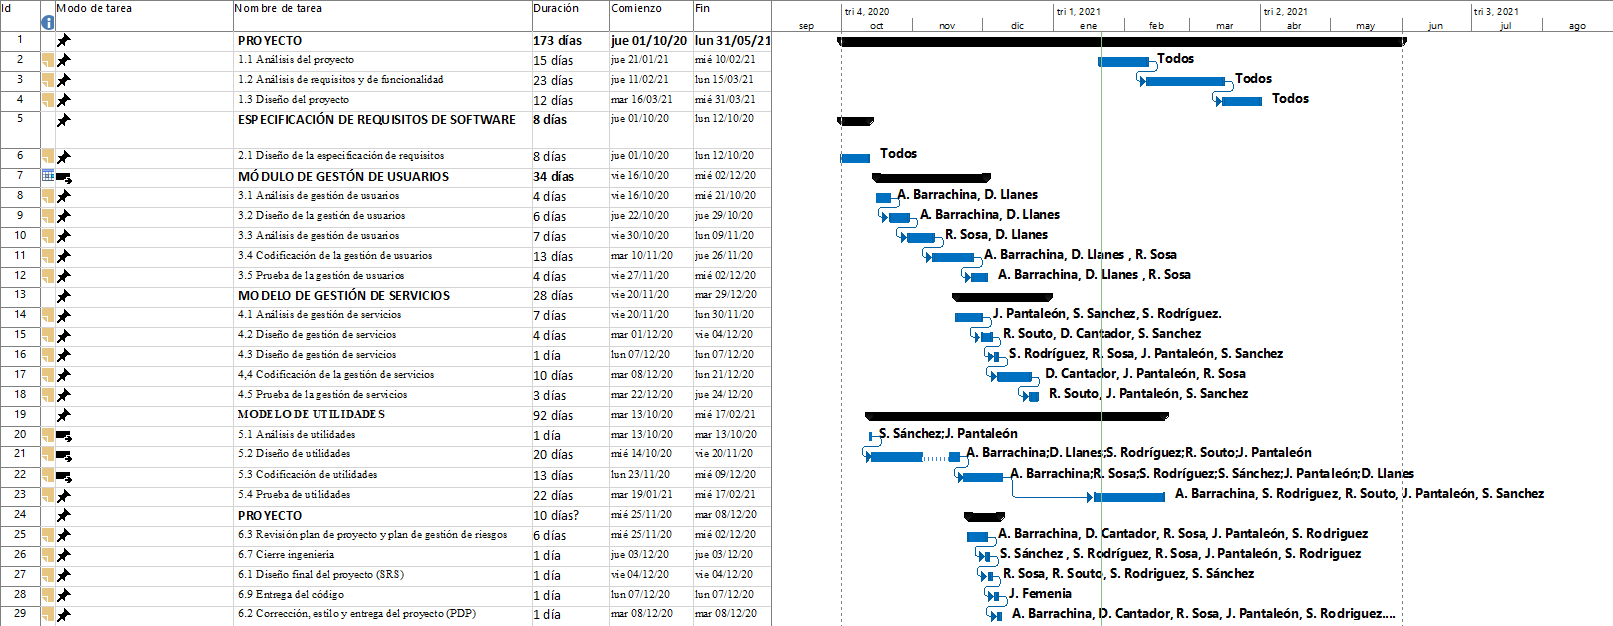
\includegraphics[width = 1.5\textwidth]{images/gantt.png}
		\caption{Diagrama de Gantt}
		\label{fig:gantt}
	\end{figure}
	\begin{figure}[H]
		\centering
		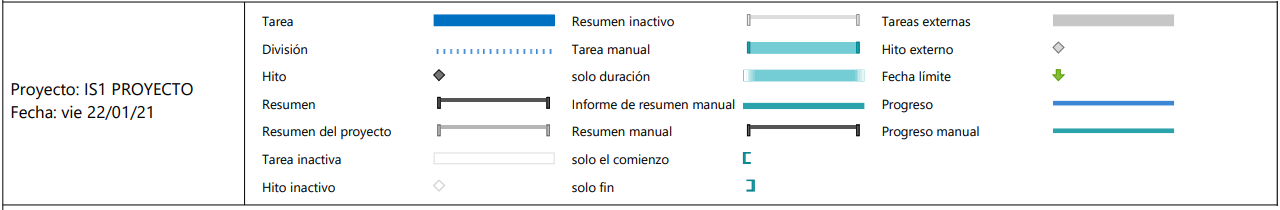
\includegraphics[width = \textwidth]{images/gantt_leyenda.PNG}
		\caption{Leyenda del diagrama \ref{fig:gantt}}
	\end{figure}
	\subsection{Red de tareas}
	\begin{figure}[H]
		\centering
		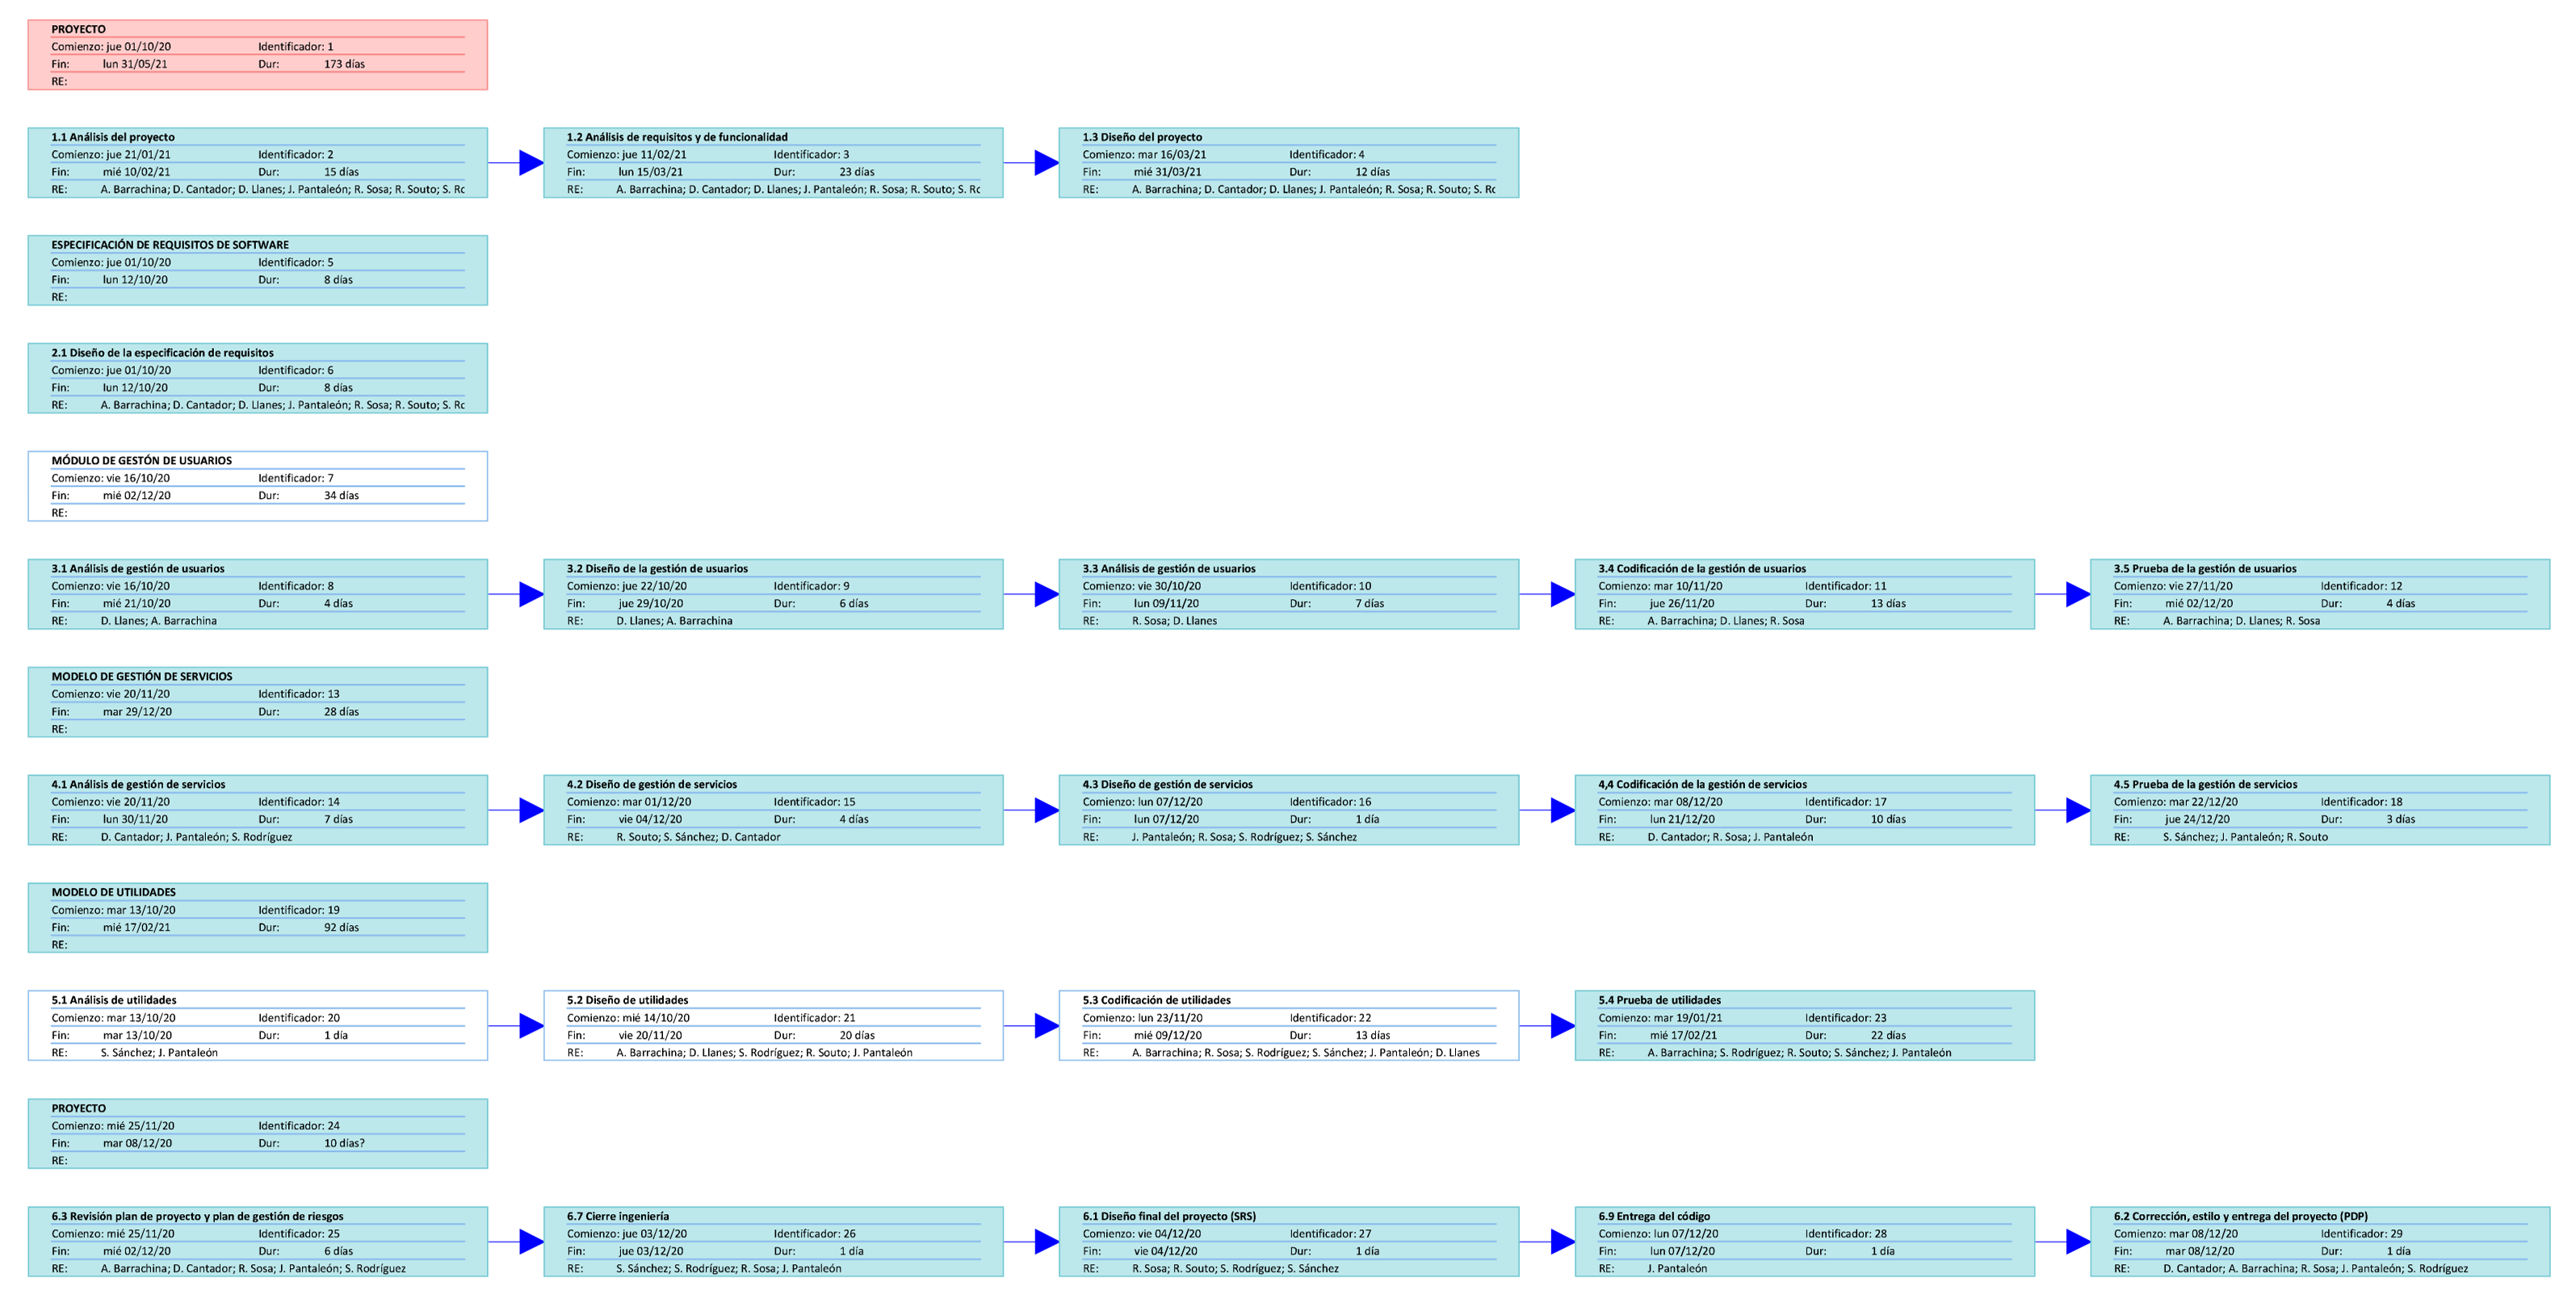
\includegraphics[width=1.5\textwidth]{images/Diagrama_Red.png}
		\caption{Diagrama en red de tareas}
	\end{figure}
\end{landscape}


\subsection{Tabla de uso de recursos}
\begin{figure}[H]
	\centering
	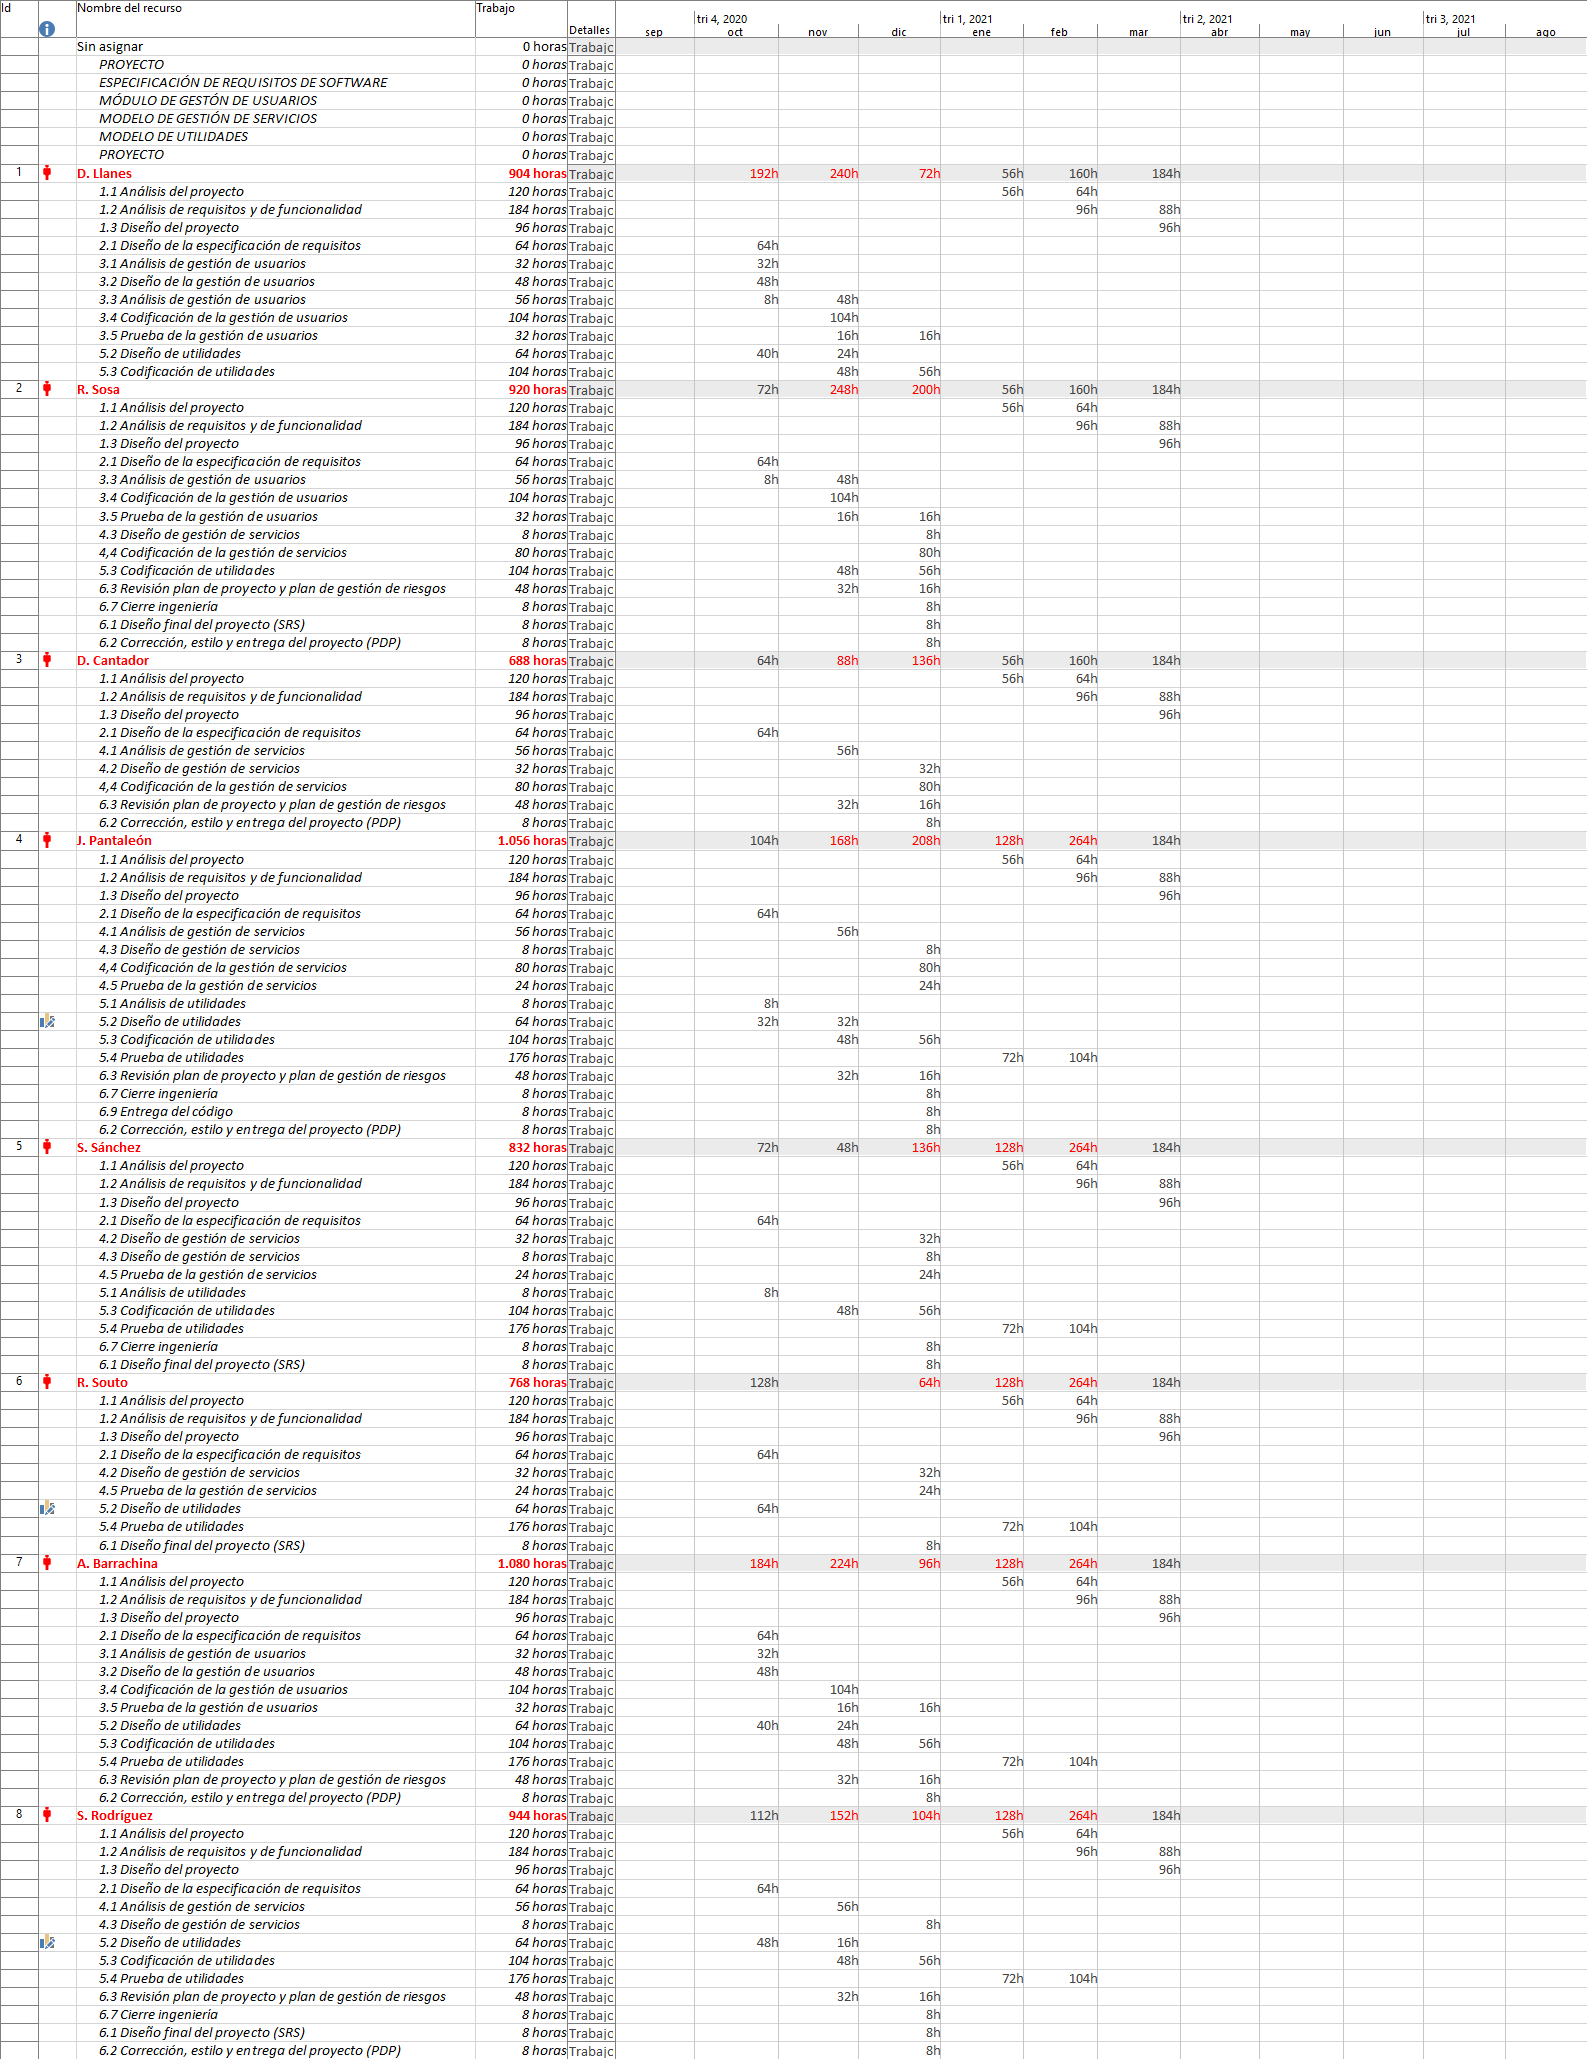
\includegraphics[width=\textwidth]{images/recursos.png}
	\caption{Uso de recursos}
\end{figure}
